\documentclass[a4paper,12pt]{scrartcl}
%test
%%%%%%%%%%%%%%%%%%%%%%%%%%%%%%%%%%%%%%%%%
\def\Nr{1}					%Hier die Nummer des Übungsblatts eintragen
\def\NameA{Dario Estermann}	%Hier den Name eintragen
\def\MatA{10054384}			%Hier die Matrikelnummer eintragen
\def\NameB{xxxxxxx}		%Hier den Name des 2. Gruppenmitglieds eintragen
\def\MatB{xxxxx}			%Hier die Matrikelnummer des 2. Gruppenmitglieds eintragen
\def\NameC{}				%Name 3. Gruppenmitglied
\def\MatC{}					%Matrikelnummer 3. Gruppenmitglied
\def\NameD{}				%Name 4. Gruppenmitglied
\def\MatD{}					%Matrikelnummer 4. Gruppenmitglied
%%%%%%%%%%%%%%%%%%%%%%%%%%%%%%%%%%%%%%%%%
\usepackage[utf8]{inputenc}
\usepackage[ngerman]{babel}
\usepackage{hyperref}
\usepackage{booktabs}
\usepackage{geometry}
\usepackage{amssymb}
\usepackage{amsmath}
\usepackage{ifthen}
\usepackage{enumerate}
\usepackage{verbatim}
\usepackage{multicol}
\usepackage{algorithm}
\usepackage{xcolor}
\setlength{\marginparwidth}{2.5cm}
\usepackage{todonotes}
\usepackage{tikz}
\usepackage{forest}
\usetikzlibrary{
	arrows,
	arrows.meta,
	automata,
	calc,
	chains,
	trees,
	positioning,
	scopes,
	decorations.pathmorphing,
	shapes,
	backgrounds,
	chains,
	}

\geometry{margin=3cm, top=2.7cm}
\renewcommand{\thesection}{\arabic{section}{.}}

\begin{document}
\begin{center}
	\sffamily
	\bfseries
	\LARGE
	Datenstrukturen und Algorithmen\\
	\Large
	\vspace{.2\parskip}
	Hausübung \Nr\\
	\normalsize\normalfont
	WiSe 23/24
	\vspace{.2\parskip}
\end{center}

\begin{tabular}[t]{p{4.5cm} p{3cm}}
	\toprule
	Name & Matrikelnummer\\
	\midrule
	\NameA & \MatA\\
	\NameB & \MatB\\
	\ifx\NameC\empty\else\NameC & \MatC\\\fi
	\ifx\NameD\empty\else\NameD & \MatD\\\fi
	\bottomrule
\end{tabular}
\hfill
\begin{tabular}[t]{ccccc}
	\toprule
	A1 & A2 & A3 & Bonus & $\Sigma$ \\
	\midrule
	\\
	\bottomrule	
\end{tabular}
\hfill\\


%%%%%%%%%%%%%%%%%%%%%%%%%%%%%%%%%%%%%%%%%%%%%%%%%%%%%%%%%%%%%%%%%%%%%%%%%%%%%%%%%%%%%%%%%
% Ab hier bearbeiten 
%%%%%%%%%%%%%%%%%%%%%%%%%%%%%%%%%%%%%%%%%%%%%%%%%%%%%%%%%%%%%%%%%%%%%%%%%%%%%%%%%%%%%%%%%
Informationen zu \LaTeX{} auf z.B.: \url{https://tex.cloud.uni-hannover.de/learn}.

\section*{Aufgabe 1}
\begin{enumerate}[a)]
	\item $f \ll g \ll h$ % inline mathmode
	\begin{enumerate}[1.]
		\item $f_3(n) = \left(\sqrt{3n} + \sqrt{12n}\right) \cdot \left(-\sqrt{3n} + \sqrt{12n}\right) = -3n + 12n = 9n = O(n)$
		\item $f_5(n) = \frac{6n^2-18n-10}{(2n+1)(n-5)} = O(n^2)$

		\item $f_2(n) = 4^{1 + \log(n^2)} + 2^{4 \cdot \log(2^n)} = O(4^{\log(n^2)})$\\
			  $\lim_{n \to \infty}4^{log(n^2)} > (2^4)^{\log(2^n)}$
		
		\item $f_4(n) = \log(9n^2) + \log(2n^5) = O(\log(n^5))$
		\item $f_6(n) = \log\left(\sqrt{2 \pi n}\left(\frac{n}{e}\right)^{\!n}\right) = O(\log(n^n))$\\
		$\lim_{n \to \infty}\log(\sqrt{n}\ n^n)$\\
		$\lim_{n \to \infty}\log(n^{n+\frac{1}{2}})$\\
		$\lim_{n \to \infty}\log(n^n)$
		
		\item $f_1(n) = 42n + 17 + 120n^2 + 23n^3 = O(n^3)$

			  
	\end{enumerate}

	\item{
		\textbf{Satz 1.22} Seien $f, g$ Funktionen. Falls $g \in O(f)$, dann folgt $f + g \in \Theta(f)$.\\
		\\hab noch nicht in \LaTeX übersetzt
	} 
\end{enumerate}

\break
\section*{Aufgabe 2}
\begin{enumerate}[a)]
	\item Gegeben ist folgender Graph. Geben Sie einen Tiefensuche-Baum von $(G, 0)$ an. 
	\begin{center}
	\begin{tikzpicture}
		\node[draw, circle] (0) {0};
		\node[draw, circle, right = of 0] (1) {1};
		\node[draw, circle, right = of 1] (2) {2};
		\node[draw, circle, below = of 0] (3) {3};
		\node[draw, circle, right = of 3] (4) {4};
		\node[draw, circle, right = of 4] (5) {5};
		\draw[-Stealth] (0) -- (1);
		\draw[-Stealth] (0) -- (3);
		\draw[-Stealth] (1) -- (5);
		\draw[-Stealth] (5) -- (2);
		\draw[-Stealth] (4) -- (1);
		\draw[-Stealth] (3) -- (1);
		\draw[-Stealth] (4) -- (0);
		\draw[-Stealth] (5) -- (4);
		\draw[-Stealth] (2) to[bend left] (5);
		\draw[-Stealth] (3) to[bend right] (5);
	\end{tikzpicture}
	\end{center}
	Tiefensuche-Baum von $(G, 0)$:
	\begin{center}
		\begin{tikzpicture}[node distance={15mm}]
			\node[draw, circle] (0){0};
			\node[draw, circle, below left of=0] (1){1};
			\node[draw, circle, below right of=0] (3){3};
			\node[draw, circle, below left of=1] (5){5};
			\node[draw, circle, below left of=5] (2){2};
			\node[draw, circle, below right of=5] (4){4};

			\draw[-Stealth] (0) -- (1);
			\draw[-Stealth] (0) -- (3);
			\draw[-Stealth] (1) -- (5);
			\draw[-Stealth] (5) -- (2);
			\draw[-Stealth] (5) -- (4);
					
		\end{tikzpicture}
		\end{center}
		\break
		\item{
			Algorithmus: Wir fangen mit den Ecken an, die nur 2 Verbindungen haben.\\
			So ist eindeutig, wenn Ecke X in A ist muss der Verbund in die Menge B!\\
			\center \begin{enumerate}[1.]
			\item Wähle 0. Verbinde 1 und 3 in B:\\
			\begin{center}
				\begin{tikzpicture}[node distance={50mm}]
					\node[label=A] (0) {0};
					\node[label=B, right of=0] (1) {1};
					\node[right of=0, below=1] (3) {3};
					
					\draw[-] (0) -- (1);
					\draw[-] (0) -- (3);
	
				\end{tikzpicture}
			\end{center}
			\item{
				Wähle 3.\\ 3 kommt wegen der Verbindung die bereits berücksichtigt wurde, in B.\\
				Die 5 als weitere Verbindung muss daher in A.\\
				\begin{center}
					\begin{tikzpicture}[node distance={50mm}]
						\node[label=A] (0) {0};
						\node[label=B, right of=0] (1) {1};
						\node[right of=0, below=1] (3) {3};
						\node[left of=3] (5) {5};
	
						\draw[-] (0) -- (1);
						\draw[-] (0) -- (3);
						\draw[-] (5) -- (3);
					\end{tikzpicture}
				\end{center}
			}
			\item{
				Wähle 1.\\ Verbindungen 2 und 4 müssen in A.\\
				\begin{center}
					\begin{tikzpicture}[node distance={50mm}]
						\node[label=A] (0) {0};
						\node[label=B, right of=0] (1) {1};
						\node[right of=0, below=1] (3) {3};
						\node[left of=3] (5) {5};
						\node[below=3] (2) {2};
						\node[below=2] (4) {4};
	
						\draw[-] (0) -- (1);
						\draw[-] (0) -- (3);
						\draw[-] (5) -- (3);
						\draw[-] (2) -- (1);
						\draw[-] (4) -- (1);
					\end{tikzpicture}
				\end{center}
			}
			\item {
				Wähle 2. Verbindungen 5 und 1 müssen in B.\\
				X Nicht möglich, durch die drei Kanten an 5 muss 5 jeweils für die anderen\\
				beiden in die gegenteilige Menge.
			}
		\end{enumerate}
	
	
		}
	\item haben wir nicht??
\end{enumerate}

\break
\section*{Aufgabe 3}
\begin{enumerate}[a)]
	\item{
	\begin{tikzpicture}[baseline=(0.center)]
		\node[draw, circle, fill=blue!33!white] (0) {0};
		\node[label=above:{Graph 1}, draw, circle, right = of 0] (1) {1};
		\node[draw, circle, right = of 1] (2) {2};
		\node[draw, circle, below = of 0] (3) {3};
		\node[draw, circle, right = of 3] (4) {4};
		\node[draw, circle, right = of 4] (5) {5};
		\draw[-] (0) -- (1);
		\draw[-] (0) -- (5);
		\draw[-] (1) -- (2);
		\draw[-] (1) -- (3);
		\draw[-] (2) -- (4);
		\draw[-] (3) -- (4);
		\draw[-] (3) to[bend right] (5);
	\end{tikzpicture}\quad\quad
	\begin{tikzpicture}[baseline=(0.center)]
		\node[draw, circle, fill=red!33!white] (0) {0};
		\node[label=above:{Graph 2}, draw, circle, right = of 0] (1) {1};
		\node[draw, circle, right = of 1] (2) {2};
		\node[draw, circle, below = of 0] (3) {3};
		\node[draw, circle, right = of 3] (4) {4};
		\node[draw, circle, right = of 4] (5) {5};
		\draw[-] (0) -- (3);
		\draw[-] (4) -- (1);
		\draw[-] (5) -- (4);
		\draw[-] (1) -- (2);
		\draw[-] (5) -- (2);
		\draw[-] (0) -- (1);
		\draw[-] (3) to[bend right] (5);
	\end{tikzpicture}\\

	\subsection*{Graph 1}
	\begin{center}
		\vspace{-5em}
		\begin{tikzpicture}
			\node[draw, circle, fill=blue!33!white] (0) {0};
			\node[draw, circle, right = of 0] (1) {1};
			\node[draw, circle, below = of 0] (2) {2};
			\node[label=below:A, draw, circle, below = of 2] (3) {3};
			\node[draw, circle, right = of 2] (4) {4};
			\node[label=below:B, draw, circle, right = of 3] (5) {5};
			\draw[-, looseness=2] (0) to[out=45, in=45] (5);
			\draw[-] (0) -- (1);
			\draw[-] (1) -- (2);
			\draw[-] (1) -- (3);
			\draw[-] (2) -- (4);
			\draw[-] (3) -- (4);
			\draw[-] (3) to[looseness=0.5, bend right] (5);
			\node[text width=10cm] at (9,-0.5) {
				Der Graph ist zweiteilbar.
				Anhand des links zu sehenden Graphen ist deutlich zu sehen, dass man den Graph so zeichnen kann, dass die Ecken der jeweiligen Mengen auf verschiedenen Seiten sind und das Kriterium vollständig erfüllt ist.  	

			};
		\end{tikzpicture}
	\end{center}
	\subsection*{Graph 2}
	Bipartitheitskriterium: Ein Graph ist genau dann zweiteilbar (oder bipartit), wenn er keinen Kreis ungerader Länge enthält.
	Hier ist aber ein Kreis der Länge von 5 enthalten, deshalb ist dieser Graph nicht zweiteilbar. 
	Der Knoten 5 hat drei Kanten, die von ihm ausgehen und somit ist die Gruppierung in eine der Mengen A oder B nicht möglich.\\
	\center 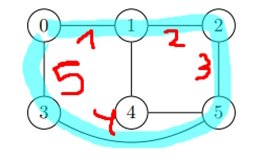
\includegraphics[scale=1] {graph2.jpg}
	}
	\pagebreak
	\item haben wir nicht??
	\item haben wir nicht??
\end{enumerate}
\end{document}